\documentclass{article}
\usepackage{tpack}

\title{ES572 - Circuitos Lógicos}
\author{Guilherme Nunes Trofino}
\authorRA{217276}
\project{Resumo Teórico}


\begin{document}
    \maketitle
\newpage

    \tableofcontents
\newpage

    \section{Introdução}
        \paragraph{Apresentação}Neste documento será descrito as informações necessárias para compreensão e solução de exercícios relacionados a disciplina \thetitle. Note que este documento são notas realizadas por \theauthor , em \today.

\begin{multicols}{2}
    \raggedcolumns

    \subsection{Informação}
        \paragraph{Definição}Informação são dados comunicados ou recebidos que resolvem incertezas sobre um fato ou circunstância específica. Assim, dada uma variável aleatória discreta $x$ com as seguintes condições:
            \begin{enumerate}[noitemsep]
                \item Possíveis Valores: $x \in \{x_{1},...,x_{n}\}$;
                \item Probabilidades Associadas: $\{p_{1},...,p_{n}\}$;
            \end{enumerate}
        Desta forma, considera-se $I(x_{i})$ que a \textbf{Quantidade de Informação Recebida}, medida em \texttt{bits}, será relacionada por:
            \begin{equation}
                \boxed{
                    I(x_{i}) = \log_{2}\left(\frac{1}{p_{i}}\right)
                }
            \end{equation}
        Nota-se trata-se de uma informação relacionada apenas ao evento analisado. Além disso, eventos de baixa probabilidade transportam mais informação.

    \columnbreak

    \subsection{Entropia}
        \paragraph{Definição}Dada uma variável aleatória $x$ então sua \textbf{Entropia} $H(x)$ será a quantidade média de informação recebida ao conhecer seu valor, sendo descrita pela equação abaixo:
            \begin{equation*}
                H(x) = E(I(x)) = \sum_{i=1}^{N}p_{i}\log_{2}\left(\frac{1}{p_{i}}\right)
            \end{equation*}
        Onde $E(x)$ representa a \textbf{Esperança} da variável $x$, podendo ser simplificada para:
            \begin{equation}
                \boxed{
                    H(x) = -\sum_{i=1}^{N}p_{i}\log_{2}p_{i}
                }
            \end{equation}
        Nota-se que trata-se de uma informação relacionada apenas ao processo analisado:
            \begin{enumerate}[noitemsep]
                \item Quanto mais baixa, mais previsível; 
                \item Quanto mais alta, mais imprevisível; 
            \end{enumerate}
\end{multicols}
        
        \subsection{Codificação}
            \paragraph{Definição}Mapeamento \textbf{biunívoco}, cada elemento associado a um único contraelemento, entre cadeias de bits e os membros do conjunto de dados a serem condificados. Classificados em:
                \begin{enumerate}[rightmargin = \leftmargin]
                    \item \textbf{Comprimento Fixo:} Caso todos os símbolos ocorram com a mesma probabilidade, geralmente utiliza-se este método;
                        \begin{enumerate}[noitemsep, rightmargin = \leftmargin]
                            \item \texttt{Vantagens:}
                                \begin{enumerate}[noitemsep, rightmargin = \leftmargin]
                                    \item Todas as folhas possuem a mesma distância da raiz;
                                    \item Acesso Aleatório: Variáveis podem ser lidas em qualquer trecho da codificação;
                                \end{enumerate}

                            \item \texttt{Entropia:} Considera-se uma variável aleatória X que assume valores entre $N$ possibilidades equiprováveis será:
                                \begin{equation}
                                    \boxed{
                                        H(x) = \sum_{i=1}^{N}p_{i}\log_{2}\left(\frac{1}{p_{i}}\right) = \sum_{i=1}^{N}\frac{1}{N}\log_{2}(N)
                                    }
                                \end{equation}
                            Desta forma, uma codificação \textbf{ótima} terá $N = 2^{k}$, onde $k \in \mathbb{N}$.
                        \end{enumerate}

                    \item \textbf{Comprimento Variável:} Caso todos os símbolos não ocorram com a mesma probabilidade, geralmente utiliza-se este método;
                        \begin{enumerate}[noitemsep, rightmargin = \leftmargin]
                            \item \texttt{Vantagens:}
                                \begin{enumerate}[noitemsep, rightmargin = \leftmargin]
                                    \item Flexibilidade para se aproximar da codificação \textbf{ideal};
                                    \item Necessária para compresão de arquivos, como descrito por \textbf{Huffman};
                                \end{enumerate}

                            \item \texttt{Entropia:} Considera-se uma variável aleatória X que assume valores entre $N$ possibilidades equiprováveis será:
                                \begin{equation}
                                    \boxed{
                                        H(x) = \sum_{i=1}^{N}p_{i}\log_{2}\left(\frac{1}{p_{i}}\right)
                                    }
                                \end{equation}
                            Desta forma, uma codificação \textbf{ótima} terá:
                                \begin{enumerate}[noitemsep, rightmargin = \leftmargin]
                                    \item \texttt{Codificação Curta:} Se $x_{i}$ tiver uma probabilidade alta;
                                    \item \texttt{Codificação Longa:} Se $x_{i}$ tiver uma probabilidade baixa;
                                \end{enumerate}
                        \end{enumerate}

                    \item \textbf{Codificação Ambígua:} Organização não única dos caracteres envolvidos o que pode gerar problemas de interpretação dos dados. Deve ser \textbf{evitada};

                \end{enumerate}
            Será necessário evitar codificações ambíguas, pois poderá haver incerteza de informação neste caso. Desta forma, uma árvore binária deve ser criada para validar se a codificação é válida, alocando as variáveis nos terminais das ramificações.

        \subsection{Algoritmo de Huffman}
            \paragraph{Definição}Algoritmo para construção de uma \textbf{Árvore Binária Ótima}, isto é uma codificação que possua entropia próxima a mínima necessária. Aplica-se os seguintes passos:
                \begin{enumerate}[rightmargin = \leftmargin]
                    \item Criação de uma sub-árvore com os símbolos de \textbf{menor} probabilidade, associando-a o somatório de suas possibilidades;
                    \item Seleção de dois símbolos ou sub-árvores com menores probabilidades e as combine em uma nova sub-árvore;
                    \begin{enumerate}[noitemsep, rightmargin = \leftmargin]
                        \item Caso hajam símbolos ou sub-árvores com mesma probabilidade, escolha arbitrariamente;
                    \end{enumerate}
                \end{enumerate}
            Consequência deste algoritmo:
                \begin{itemize}[rightmargin = \leftmargin]
                    \item Todas as codificações apresentam o mesmo comprimento esperado, logo a mesma eficiência, independente dos rótulos empregados para cada ramificação;
                    \item Desempenhos mais próximos da entropia podem ser obtidos com sequências maiores, normalmente aplicadas em algoritmos de compressão como \texttt{LZW};
                \end{itemize}

    \begin{multicols}{2}
        \begin{figure}[H]
            \centering
            \begin{forest} % from https://tex.stackexchange.com/a/304002/121799
                for tree={
                    s sep = 10mm,   % Horizontal Distance
                    l = 0mm,        % Vertical Distance
                    where n children={0}{ev}{iv},
                    l+=8mm,
                    if n=1{
                        edge label={
                            node [midway, left] {0}
                        }
                    }{
                        edge label={
                            node [midway, right] {1}
                        }
                    }
                }
                [100
                    [60
                        [A] [B]
                    ]
                    [40
                        [C]
                        [20
                            [D] [E]
                        ]
                    ]
                ]
            \end{forest}
            \caption{Representação da Árvore de Huffman}
        \end{figure} \noindent

        \columnbreak\noindent
        Considera-se como exemplo a seguinte distribuição de probabilidades:
            \begin{table}[H]
                \centering
                \begin{tabular}[]{ccc}\hline
                    Símbolos & Probabilidade & Codificação\\\hline
                    A & 30 & 00\\
                    B & 30 & 01\\
                    C & 20 & 10\\
                    D & 10 & 110\\
                    E & 10 & 111\\\hline
                \end{tabular}
                \caption{Probabilidades dos Símbolos}\label{table:Huffman}
            \end{table}
    \end{multicols}

        \subsection{Distância de Hamming}
            \paragraph{Definição}Representa o número de posições nos quais os dígitos correspondentes \textbf{diferem} entre si, como representado abaixo:
                \begin{table}[H]
                    \centering
                    \begin{tabular}[]{cc}\hline
                        Original  & Palavra Código\\\hline
                        0110 0100 & 01\textcolor{red}{0}0 \textcolor{red}{1}100\\\hline
                    \end{tabular}
                    \caption{Representação da Distância de Hamming}\label{table:HammingDefinition}
                \end{table}\noindent

        \subsubsection{Deteção de \texttt{Erro de 1 bit}}
            \paragraph{Definição}Criação de palavras código válidas, de modo que um erro de um \textbf{único} \texttt{bit} não produza outra palavra de código válida. Desta forma, será necessário uma codificação cuja distância de Hamming entre quaisquer palavras válidas seja de \textbf{pelo menos} 2.

            \paragraph{Aplicação}Adiciona-se um \texttt{bit} em qualquer palavra válida para que o número total de \texttt{bits 1} seja:
                \begin{enumerate}[noitemsep, rightmargin = \leftmargin]
                    \item \textbf{Paridade Par:} Possui um número par de \texttt{bits 1}. Representado com \texttt{bit 0};
                    \item \textbf{Paridade Ímpar:} Possui um número ímpar de \texttt{bits 1}. Representado com \texttt{bit 1};
                \end{enumerate}

            \paragraph{Generalização}Considere um símbolo codificado qualquer, para \textbf{Detectar} um número $E$ de erros será necessário uma distância mínima de Hamming $E+1$ entre as palavras de código. Além disso, a \textbf{Correção} um número $E$ de erros será necessário uma distância mínima de Hamming $2E+1$.

        \subsubsection{Codificação de Hamming \texttt{(15, 11)}}
            \paragraph{Definição}Organização de dados em \texttt{15 bits}, \texttt{11 bits} de dados e \texttt{4 bits} são redundância. Desta forma, os \texttt{bits} redundantes são suficientes para determinar a posição de qualquer erro de \texttt{1 bit} presente nos dados.

            \paragraph{Aplicação}Organize os \texttt{11 bits} de dados sequencialmente nos espaços brancos de uma matriz 4x4 como representado abaixo:
                \begin{table}[H]
                    \centering\begin{tabular}{|c|c|c|c|}\hline
                        \cellcolor{blue!40}\mycell{x}{0} & \cellcolor{red!40}\mycell{p}{1} & \cellcolor{red!40}\mycell{p}{2}  & \mycell{1}{3}\\\hline
                        \cellcolor{red!40}\mycell{p}{4}  & \mycell{0}{5}                   & \mycell{1}{6}                    & \mycell{0}{7}\\\hline
                        \cellcolor{red!40}\mycell{p}{8}  & \mycell{0}{9}                   & \mycell{1}{10}                   & \mycell{0}{11}\\\hline
                        \mycell{1}{12}                   & \mycell{0}{13}                  & \mycell{0}{14}                   & \mycell{1}{15}\\\hline
                    \end{tabular}
                    \caption{Codificação de Hamming}
                    \label{table:HammingCode}
                \end{table}\noindent
            Na sequência preenche-se os \textcolor{red!80}{\texttt{bits de paridade}}, apresentados nas posições com \textcolor{red!80}{p}, representando a paridade de cada \textbf{subgrupo} possuam como representado abaixo:
                \begin{table}[H]
                    \centering
                    \begin{tabular}{|c|c|c|c|}\hline
                        \mycell{x}{0}  & \cellcolor{red!40}\mycell{0}{1}   & \mycell{p}{2}  & \cellcolor{gray!50}\mycell{1}{3}\\\hline
                        \mycell{p}{4}  & \cellcolor{gray!50}\mycell{0}{5}  & \mycell{1}{6}  & \cellcolor{gray!50}\mycell{0}{7}\\\hline
                        \mycell{p}{8}  & \cellcolor{gray!50}\mycell{0}{9}  & \mycell{1}{10} & \cellcolor{gray!50}\mycell{0}{11}\\\hline
                        \mycell{1}{12} & \cellcolor{gray!50}\mycell{0}{13} & \mycell{0}{14} & \cellcolor{gray!50}\mycell{1}{15}\\\hline
                    \end{tabular}
                    \quad
                    \begin{tabular}{|c|c|c|c|}\hline
                        \mycell{x}{0}  & \mycell{0}{1}  & \cellcolor{red!40}\mycell{0}{2}   & \cellcolor{gray!50}\mycell{1}{3}\\\hline
                        \mycell{p}{4}  & \mycell{0}{5}  & \cellcolor{gray!50}\mycell{1}{6}  & \cellcolor{gray!50}\mycell{0}{7}\\\hline
                        \mycell{p}{8}  & \mycell{0}{9}  & \cellcolor{gray!50}\mycell{1}{10} & \cellcolor{gray!50}\mycell{0}{11}\\\hline
                        \mycell{1}{12} & \mycell{0}{13} & \cellcolor{gray!50}\mycell{0}{14} & \cellcolor{gray!50}\mycell{1}{15}\\\hline
                    \end{tabular}
                    \quad
                    \begin{tabular}{|c|c|c|c|}\hline
                        \mycell{x}{0}                     & \mycell{0}{1}                     & \mycell{0}{2}                     & \mycell{1}{3}\\\hline
                        \cellcolor{red!40}\mycell{1}{4}   & \cellcolor{gray!50}\mycell{0}{5}  & \cellcolor{gray!50}\mycell{1}{6}  & \cellcolor{gray!50}\mycell{0}{7}\\\hline
                        \mycell{p}{8}                     & \mycell{0}{9}                     & \mycell{1}{10}                    & \mycell{0}{11}\\\hline
                        \cellcolor{gray!50}\mycell{1}{12} & \cellcolor{gray!50}\mycell{0}{13} & \cellcolor{gray!50}\mycell{0}{14} & \cellcolor{gray!50}\mycell{1}{15}\\\hline
                    \end{tabular}
                    \quad
                    \begin{tabular}{|c|c|c|c|}\hline
                        \mycell{x}{0}                     & \mycell{0}{1}                     & \mycell{0}{2}                     & \mycell{1}{3}\\\hline
                        \mycell{1}{4}                     & \mycell{0}{5}                     & \mycell{1}{6}                     & \mycell{0}{7}\\\hline
                        \cellcolor{red!40}\mycell{1}{8}   & \cellcolor{gray!50}\mycell{0}{9}  & \cellcolor{gray!50}\mycell{1}{10} & \cellcolor{gray!50}\mycell{0}{11}\\\hline
                        \cellcolor{gray!50}\mycell{1}{12} & \cellcolor{gray!50}\mycell{0}{13} & \cellcolor{gray!50}\mycell{0}{14} & \cellcolor{gray!50}\mycell{1}{15}\\\hline
                    \end{tabular}
                    \caption{Grupos de Hamming}
                    \label{table:HammingGroups}
                \end{table}\noindent
            Neste ponto pode-se detectar e localizar \texttt{erros de 1 bit}. Na sequência preenche-se o \textcolor{blue!80}{\texttt{bit de paridade do conjunto}} para paridade do \textbf{grupo} como representado abaixo:
                \begin{table}[H]
                    \centering
                    \begin{tabular}{|c|c|c|c|}\hline
                        \cellcolor{blue!40}\mycell{1}{0} & \mycell{0}{1}  & \mycell{0}{2}  & \mycell{1}{3}\\\hline
                        \mycell{1}{4}                    & \mycell{0}{5}  & \mycell{1}{6}  & \mycell{0}{7}\\\hline
                        \mycell{1}{8}                    & \mycell{0}{9}  & \mycell{1}{10} & \mycell{0}{11}\\\hline
                        \mycell{1}{12}                   & \mycell{0}{13} & \mycell{0}{14} & \mycell{1}{15}\\\hline
                    \end{tabular}
                    \caption{Codificação Hamming Estendida}
                    \label{table:HammingFinal}
                \end{table}\noindent
            Neste ponto pode-se localizar \texttt{erros de 2 bits}.

        \subsubsection{Decodificação de Hamming \texttt{(15, 11)}}
            \paragraph{Definição}Interpretação dos dados recebidos na \textbf{Configuração de Hamming}, analisando os \texttt{15, ou 16, bits} codificados como descrito abaixo:
                \begin{enumerate}[rightmargin = \leftmargin]
                    \item \textbf{Transmissão Correta:} 
                        \begin{enumerate}[noitemsep, rightmargin = \leftmargin]
                            \item Não houve erro nos \textcolor{red!80}{\texttt{bits de paridade}};
                            \item Não houve erro no \textcolor{blue!80}{\texttt{bit de paridade do conjunto}};
                        \end{enumerate}

                    \item \textbf{Transmissão com} \texttt{Erro de 1 bit}:
                        \begin{enumerate}[noitemsep, rightmargin = \leftmargin]
                            \item Houve erro em pelo menos um dos \textcolor{red!80}{\texttt{bits de paridade}};
                            \item Houve erro no \textcolor{blue!80}{\texttt{bit de paridade do conjunto}};
                        \end{enumerate}

                    \item \textbf{Transmissão com} \texttt{Erro de 2 bit}:
                        \begin{enumerate}[noitemsep, rightmargin = \leftmargin]
                            \item Houve erro em pelo menos um dos \textcolor{red!80}{\texttt{bits de paridade}};
                            \item Não houve erro no \textcolor{blue!80}{\texttt{bit de paridade do conjunto}};
                        \end{enumerate}
                \end{enumerate}

    \section{Abstração Digital}
        \paragraph{Apresentação}Depois de discutido como codificar informações como sequência de bits será necessário elaborar uma forma para codifica-la fisicamente que atenda aos seguintes características:
            \begin{enumerate}[noitemsep]
                \item \textbf{Pequeno:} Necessite de pouco espaço para armazenamento;
                \item \textbf{Barato:} Economicamente acessível para produção;
                \item \textbf{Estável:} Não apresentará mudanças durante seu uso;
                \item \textbf{Veloz:} Fácil de acessar, transformar, combinar, transmitir e armazenar;
            \end{enumerate}
        No mundo, não quântico, não é digital e são afetados por imperfeições que devem ser consideradas na descrição de modelo de conversão que consigo manter a precisão necessária para aplicação desejada.

        \subsection{Processamento Digital}
            \paragraph{Definição}Conversão, manipulação e utilização de sinais digitais para interpretação de fenômenos físicos estudados. Isso demandará algumas definições de conceitos descritas na sequência.

            \subsubsection{Conversão Digital}
                \paragraph{Definição}Inicialmente será necessário determinar como os sinais analógicos, medições reais, serão convertido para sinais digitais para que então possam ser trabalhados, buscando métodos que atendam as condições de codificações como a representada a seguir:
                    \begin{figure}[H]
                        \centering
                        \begin{tikzpicture}
                            \draw[-{Latex[round]}] (-0.5,0) -- (10.5,0) node[right] {volts};
                    
                            \draw[
                                color   =red!75,
                                fill    =red!25,
                                opacity =0.25
                            ] (2.5,0) 
                            node[
                                below, 
                                text=black, 
                                opacity=1
                            ] {$V_{OL}$} 
                            rectangle (3.5, 1);
                    
                            \draw[
                                color   =gray!75,
                                fill    =gray!25,
                                opacity =0.25
                            ] (3.5,0) 
                            node[
                                below, 
                                text=black, 
                                opacity=1
                            ] {$V_{IL}$} 
                            rectangle (6.5, 1) 
                            node[
                                pos=.5, 
                                text=black, 
                                opacity=1
                            ] {Zona Proibida};
                    
                            \draw[
                                color   =red!75,
                                fill    =red!25,
                                opacity =0.25
                            ] (6.5,0) 
                            node[
                                below, 
                                text=black, 
                                opacity=1
                            ] {$V_{IH}$}
                            rectangle (7.5, 1);
                    
                            \node[below] at (7.5,0) {$V_{OH}$};
                    
                            \node at ( 1.25,0.5) {0 Válido};
                            \node at ( 8.75,0.5) {1 Válido};
                    
                            \draw[
                                red,
                                decorate,
                                decoration = {
                                    brace, 
                                    mirror, 
                                    amplitude   = 2pt,
                                    raise       = 2pt
                                }
                            ] (6.5, -0.5) -- (7.5, -0.5);
                            \draw[
                                red,
                                decorate,
                                decoration = {
                                    brace, 
                                    mirror, 
                                    amplitude   = 2pt,
                                    raise       = 2pt
                                }
                            ] (2.5, -0.5) -- (3.5, -0.5);
                            \node[red] at (5,-1) {Margem de Ruído};
                    
                            \draw[
                                decorate,
                                decoration = {
                                    brace, 
                                    mirror, 
                                    amplitude   = 2pt,
                                    raise       = 2pt
                                }
                            ] (0, -0.5) -- (2.5, -0.5) node[black, midway,yshift=-0.5cm] {Saída Válida};
                            \draw[
                                decorate,
                                decoration = {
                                    brace, 
                                    mirror, 
                                    amplitude   = 2pt,
                                    raise       = 2pt
                                }
                            ] (7.5, -0.5) -- (10, -0.5) node[black, midway,yshift=-0.5cm] {Saída Válida};
                    
                            \draw[
                                decorate,
                                decoration = {
                                    brace, 
                                    amplitude   = 2pt,
                                    raise       = 2pt
                                }
                            ] (0, 1) -- (3.5, 1) node[black, midway,yshift=0.5cm] {Entrada Válida};
                            \draw[
                                decorate,
                                decoration = {
                                    brace, 
                                    amplitude   = 2pt,
                                    raise       = 2pt
                                }
                            ] (6.5, 1) -- (10, 1) node[black, midway,yshift=0.5cm] {Entrada Válida};
                        \end{tikzpicture}
                    \end{figure}\noindent

                    \begin{figure}[H]
                        \centering
                        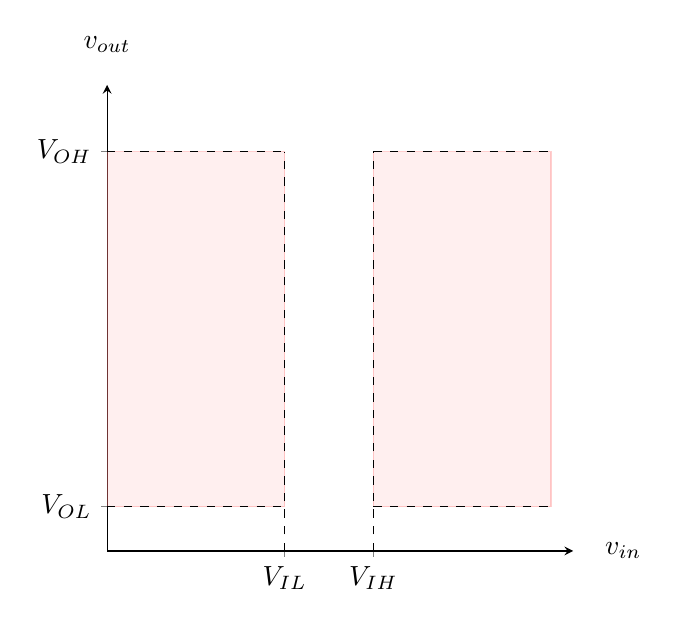
\begin{tikzpicture}
                            \begin{axis}[
                                xmin = 0, xmax = 5.25, % Axis Coordenates
                                ymin = 0, ymax = 5.25, % Axis Coordenates
                                xlabel = {$v_{\text{in}}$},  % Axis Labels
                                ylabel = {$v_{\text{out}}$}, % Axis Labels
                                xtick = {2,3},      % Axis Ticks Potions
                                ytick = {0.5,4.5},  % Axis Ticks Potions
                                xticklabels = {$V_{IL}$, $V_{IH}$}, % Axis Ticks Labels
                                yticklabels = {$V_{OL}$, $V_{OH}$}, % Axis Ticks Labels
                                x label style = {at={(axis cs:{5.5,0})}, anchor=west},
                                y label style = {at={(axis cs:{0,5.5})}, anchor=south, rotate=-90},
                                width  = 7.5cm,
                                height = 7.5cm,
                                % grid = both,
                                % grid style       = {line width=.1pt, draw=gray!10},
                                % major grid style = {line width=.2pt, draw=gray!50},
                                % minor tick num=1,
                                axis lines = left,
                            ]
                            \draw[
                                color   =red!75,
                                fill    =red!25,
                                opacity =0.25
                            ] (3,0.5) rectangle (5, 4.5);
                            \draw[
                                color   =red!75,
                                fill    =red!25,
                                opacity =0.25
                            ] (0,0.5) rectangle (2, 4.5);
                            \draw[dashed] (axis cs:{2,0}) -- (axis cs:{2,4.5});
                            \draw[dashed] (axis cs:{3,0}) -- (axis cs:{3,4.5});
                            \draw[dashed] (axis cs:{0,0.5}) -- (axis cs:{2,0.5});
                            \draw[dashed] (axis cs:{3,0.5}) -- (axis cs:{5,0.5});
                            \draw[dashed] (axis cs:{0,4.5}) -- (axis cs:{2,4.5});
                            \draw[dashed] (axis cs:{3,4.5}) -- (axis cs:{5,4.5});
                            \end{axis}
                        \end{tikzpicture}
                    \end{figure}\noindent

\newpage
        \subsubsection{Atraso de Propagação, $t_{PD}$}
            \paragraph{Definição}Limitante superior para o atraso de entradas válidas para saídas válidas causado pela presença intrínseca de capacitâncias e resistências na construção dos dispositivos como representado pelo seguinte gráfico:
                \begin{figure}[H]
                    \centering
                    \begin{tikzpicture}
                        \begin{axis}[
                            xmin = 0, xmax = 15.25, % Axis Coordenates
                            ymin = 0, ymax = 5.25, % Axis Coordenates
                            xlabel = {$t$},  % Axis Labels
                            ylabel = {$v_{\text{in}}$}, % Axis Labels
                            xtick = {5,10.75},      % Axis Ticks Potions
                            ytick = {1,04},  % Axis Ticks Potions
                            xticklabels = {$t_{1}$,$t_{2}$}, % Axis Ticks Labels
                            yticklabels = {$V_{IL}$, $V_{IH}$}, % Axis Ticks Labels
                            x label style = {at={(axis cs:{15.5,0})}, anchor=west},
                            y label style = {at={(axis cs:{0,5.5})}, anchor=south, rotate=-90},
                            width  = 15.0cm,
                            height =  4.0cm,
                            axis lines = left,
                        ]
                        \draw[] (axis cs:{0,0.5}) -- (axis cs:{4.125,0.5});
                        \draw[] (axis cs:{4.125,0.5}) -- (axis cs:{5.125,4.5});
                
                        \draw[] (axis cs:{5.125,4.5}) -- (axis cs:{9.875,4.5});
                        \draw[] (axis cs:{9.875,4.5}) -- (axis cs:{10.875,0.5});
                
                        \draw[] (axis cs:{10.875,0.5}) -- (axis cs:{14.5,0.5});
                
                        \draw[red, dashed] (axis cs:{05,0}) -- (axis cs:{05,5.5});
                        \draw[red, dashed] (axis cs:{10.75,0}) -- (axis cs:{10.75,5.5});
                        \draw[gray, dashed] (axis cs:{0,1}) -- (axis cs:{15,1});
                        \draw[gray, dashed] (axis cs:{0,4}) -- (axis cs:{15,4});
                        \end{axis}
                    \end{tikzpicture}
                    \begin{tikzpicture}
                        \begin{axis}[
                            xmin = 0, xmax = 15.25, % Axis Coordenates
                            ymin = 0, ymax = 5.25, % Axis Coordenates
                            xlabel = {$t$},  % Axis Labels
                            ylabel = {$v_{\text{out}}$}, % Axis Labels
                            xtick = {5.875,11.625},      % Axis Ticks Potions
                            ytick = {1,04},  % Axis Ticks Potions
                            xticklabels = {$t_{3}$,$t_{4}$}, % Axis Ticks Labels
                            yticklabels = {$V_{OL}$, $V_{OH}$}, % Axis Ticks Labels
                            x label style = {at={(axis cs:{15.5,0})}, anchor=west},
                            y label style = {at={(axis cs:{0,5.5})}, anchor=south, rotate=-90},
                            width  = 15.0cm,
                            height =  4.0cm,
                            axis lines = left,
                        ]
                        \draw[] (axis cs:{0,4.5}) -- (axis cs:{5,4.5});
                        \draw[] (axis cs:{5,4.5}) -- (axis cs:{6,0.5});
                
                        \draw[] (axis cs:{6,0.5}) -- (axis cs:{10.75,0.5});
                        \draw[] (axis cs:{10.75,0.5}) -- (axis cs:{11.75,4.5});
                
                        \draw[] (axis cs:{11.75,4.5}) -- (axis cs:{14.5,4.5});
                
                        \draw[red, dashed] (axis cs:{5.875,0}) -- (axis cs:{5.875,5.5});
                        \draw[red, dashed] (axis cs:{11.625,0}) -- (axis cs:{11.625,5.5});
                        \draw[gray, dashed] (axis cs:{0,1}) -- (axis cs:{15,1});
                        \draw[gray, dashed] (axis cs:{0,4}) -- (axis cs:{15,4});
                
                        \draw[{Latex[round]}-{Latex[round]}] (axis cs:{5,5}) -- (axis cs:{5.875,5});
                        \draw[{Latex[round]}-{Latex[round]}] (axis cs:{10.75,5}) -- (axis cs:{11.625,5});
                        \end{axis}
                        \node[above] at ( 5,2.5) {$t_{PD}$};
                        \node[above] at (10,2.5) {$t_{PD}$};
                    \end{tikzpicture}
                    \caption{Atraso de Propagação}
                \end{figure}\noindent
            Note que os circuitos não serão necessariamente simétricos e portanto o $t_{PD}$ do dispositivo será o \textbf{máximo} entre os atrasos de propagação como mostrado pela seguinte equação:
                \begin{equation}
                    \boxed{
                        t_{PD} = \max\{ (t_{3} - t_{1}), (t_{4} - t_{2}) \}
                    }
                \end{equation}

        \subsubsection{Atraso de Contaminação, $t_{CD}$}
            \paragraph{Definição}Limitante inferior para o atraso de entradas inválidas para saídas inválidas causado pela presença intrínseca de ruídos ou interferência na atuação dos dispositivos como representado pelo seguinte gráfico:
                \begin{figure}[H]
                    \centering
                    \begin{tikzpicture}
                        \begin{axis}[
                            xmin = 0, xmax = 15.25, % Axis Coordenates
                            ymin = 0, ymax = 5.25, % Axis Coordenates
                            xlabel = {$t$},  % Axis Labels
                            ylabel = {$v_{\text{in}}$}, % Axis Labels
                            xtick = {4.25,10.0},      % Axis Ticks Potions
                            ytick = {1,04},  % Axis Ticks Potions
                            xticklabels = {$t_{1}$,$t_{2}$}, % Axis Ticks Labels
                            yticklabels = {$V_{IL}$, $V_{IH}$}, % Axis Ticks Labels
                            x label style = {at={(axis cs:{15.5,0})}, anchor=west},
                            y label style = {at={(axis cs:{0,5.5})}, anchor=south, rotate=-90},
                            width  = 15.0cm,
                            height =  4.0cm,
                            axis lines = left,
                        ]
                        \draw[] (axis cs:{0,0.5}) -- (axis cs:{4.125,0.5});
                        \draw[] (axis cs:{4.125,0.5}) -- (axis cs:{5.125,4.5});
                
                        \draw[] (axis cs:{5.125,4.5}) -- (axis cs:{9.875,4.5});
                        \draw[] (axis cs:{9.875,4.5}) -- (axis cs:{10.875,0.5});
                
                        \draw[] (axis cs:{10.875,0.5}) -- (axis cs:{14.5,0.5});
                
                        \draw[red, dashed] (axis cs:{4.25,0}) -- (axis cs:{4.25,5.5});
                        \draw[red, dashed] (axis cs:{10.0,0}) -- (axis cs:{10.0,5.5});
                        \draw[gray, dashed] (axis cs:{0,1}) -- (axis cs:{15,1});
                        \draw[gray, dashed] (axis cs:{0,4}) -- (axis cs:{15,4});
                        \end{axis}
                    \end{tikzpicture}
                    \begin{tikzpicture}
                        \begin{axis}[
                            xmin = 0, xmax = 15.25, % Axis Coordenates
                            ymin = 0, ymax = 5.25, % Axis Coordenates
                            xlabel = {$t$},  % Axis Labels
                            ylabel = {$v_{\text{out}}$}, % Axis Labels
                            xtick = {5.125,10.875},      % Axis Ticks Potions
                            ytick = {1,04},  % Axis Ticks Potions
                            xticklabels = {$t_{1}$,$t_{2}$}, % Axis Ticks Labels
                            yticklabels = {$V_{OL}$, $V_{OH}$}, % Axis Ticks Labels
                            x label style = {at={(axis cs:{15.5,0})}, anchor=west},
                            y label style = {at={(axis cs:{0,5.5})}, anchor=south, rotate=-90},
                            width  = 15.0cm,
                            height =  4.0cm,
                            axis lines = left,
                        ]
                        \draw[] (axis cs:{0,4.5}) -- (axis cs:{5,4.5});
                        \draw[] (axis cs:{5,4.5}) -- (axis cs:{6,0.5});
                
                        \draw[] (axis cs:{6,0.5}) -- (axis cs:{10.75,0.5});
                        \draw[] (axis cs:{10.75,0.5}) -- (axis cs:{11.75,4.5});
                
                        \draw[] (axis cs:{11.75,4.5}) -- (axis cs:{14.5,4.5});
                
                        \draw[red, dashed] (axis cs:{5.125,0}) -- (axis cs:{5.125,5.5});
                        \draw[red, dashed] (axis cs:{10.875,0}) -- (axis cs:{10.875,5.5});
                        \draw[gray, dashed] (axis cs:{0,1}) -- (axis cs:{15,1});
                        \draw[gray, dashed] (axis cs:{0,4}) -- (axis cs:{15,4});
                
                        \draw[{Latex[round]}-{Latex[round]}] (axis cs:{4.25,5}) -- (axis cs:{5.125,5});
                        \draw[{Latex[round]}-{Latex[round]}] (axis cs:{10.0,5}) -- (axis cs:{10.875,5});
                        \end{axis}
                        \node[above] at (4.25,2.5) {$t_{CD}$};
                        \node[above] at (9.25,2.5) {$t_{CD}$};
                    \end{tikzpicture}
                    \caption{Atraso de Contaminação}
                \end{figure}\noindent
            Note que os circuitos não serão necessariamente simétricos e portanto o $t_{CD}$ do dispositivo será o \textbf{mínimo} entre os atrasos de propagação como mostrado pela seguinte equação:
                \begin{equation}
                    \boxed{
                        t_{CD} = \min\{ (t_{3} - t_{1}), (t_{4} - t_{2}) \}
                    }
                \end{equation}
\newpage
        \subsection{Dispositivos Combinacionais}
            \paragraph{Definição}Componente eletrônico que atende as seguintes especificações:
                \begin{enumerate}[rightmargin = \leftmargin]
                    \item \textbf{Comunicação:} Necessidades para interface com o dispositivo apresentando:
                        \begin{enumerate}[noitemsep]
                            \item \texttt{Entradas:} Ao menos uma entrada digital;
                            \item \texttt{Saídas:} Ao menos uma saída digital;
                        \end{enumerate}

                    \item \textbf{Especificação Funcional:} Qualquer saída será obtida por uma combinação possível das entradas válidas;

                    \item \textbf{Especificação Temporal:} Há um \texttt{Tempo de Propagação} $t_{PD}$ mínimo necessário para que o dispositivo calcule a saída a partir de suas entradas válidas;
                \end{enumerate}
            Além disso, um conjunto de elementos interconectados será combinacional se não viola nenhuma das seguintes regras:
                \begin{enumerate}[noitemsep]
                    \item \textbf{Condição 1:} Cada elemento individual é combinacional;

                    \item \textbf{Condição 2:} Cada entrada é conectada a uma, e apenas uma, saída ou fornecimento externo;

                    \item \textbf{Condição 3:} Não há ciclos diretos;
                \end{enumerate}

        \subsubsection{Buffer}
            \paragraph{Definição}Dispositivo eletrônico que transfere tensão, mantendo sua estabilidade apesar de logicamente não alterá-lo visto que ao longo da transmisssão o acumulo de ruídos poderia modificar o sinal transmitido.

            \paragraph{Representação}Dispositivo apresentará a seguinte tabela verdade e representação em circuitos:
                \begin{multicols}{2}
                    \begin{table}[H]
                        \centering  
                        \begin{tabular}[]{c|c}\hline
                            in & out\\\hline
                            0  & 0\\
                            1  & 1\\\hline
                        \end{tabular}
                        \caption{Tabela Verdade Buffer}
                    \end{table}
                    \columnbreak\noindent
                    \begin{figure}[H]
                        \centering
                        \begin{circuitikz}
                            \ctikzset{component text=left}
                            \draw
                            (0,0) node[buffer] (myPort) {}
                            (myPort.in)  node [anchor = east] {in}
                            (myPort.out) node [anchor = west] {out};
                        \end{circuitikz} 
                        \caption{Representação Buffer}
                    \end{figure} \noindent
                \end{multicols}\noindent
            Além disso, a representação da \textbf{Curva Característica de Transferência}, relação entre a tensão de entrada com a tensão de saída, será dada pelo seguinte gráfico:
                \begin{figure}[H]
                    \centering
                    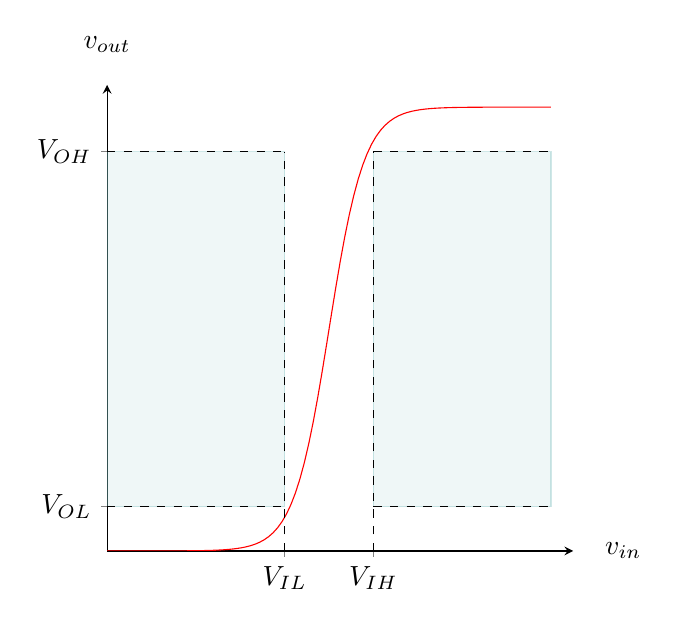
\begin{tikzpicture}
                        \begin{axis}[
                            xmin = 0, xmax = 5.25, % Axis Coordenates
                            ymin = 0, ymax = 5.25, % Axis Coordenates
                            xlabel = {$v_{\text{in}}$},  % Axis Labels
                            ylabel = {$v_{\text{out}}$}, % Axis Labels
                            xtick = {2,3},      % Axis Ticks Potions
                            ytick = {0.5,4.5},  % Axis Ticks Potions
                            xticklabels = {$V_{IL}$, $V_{IH}$}, % Axis Ticks Labels
                            yticklabels = {$V_{OL}$, $V_{OH}$}, % Axis Ticks Labels
                            x label style = {at={(axis cs:{5.5,0})}, anchor=west},
                            y label style = {at={(axis cs:{0,5.5})}, anchor=south, rotate=-90},
                            width  = 7.5cm,
                            height = 7.5cm,
                            % grid = both,
                            % grid style       = {line width=.1pt, draw=gray!10},
                            % major grid style = {line width=.2pt, draw=gray!50},
                            % minor tick num=1,
                            axis lines = left,
                        ]
                        \addplot [
                                domain=0:5, 
                                samples=100, 
                                color=red,
                        ] {5/(1+exp(-5*x+12.5))};
                        \draw[
                            color   =teal!75,
                            fill    =teal!25,
                            opacity =0.25
                        ] (3,0.5) rectangle (5, 4.5);
                        \draw[
                            color   =teal!75,
                            fill    =teal!25,
                            opacity =0.25
                        ] (0,0.5) rectangle (2, 4.5);
                        \draw[dashed] (axis cs:{2,0}) -- (axis cs:{2,4.5});
                        \draw[dashed] (axis cs:{3,0}) -- (axis cs:{3,4.5});
                        \draw[dashed] (axis cs:{0,0.5}) -- (axis cs:{2,0.5});
                        \draw[dashed] (axis cs:{3,0.5}) -- (axis cs:{5,0.5});
                        \draw[dashed] (axis cs:{0,4.5}) -- (axis cs:{2,4.5});
                        \draw[dashed] (axis cs:{3,4.5}) -- (axis cs:{5,4.5});
                        \end{axis}
                    \end{tikzpicture}
                \end{figure}\noindent
            Note que este gráfico não apresenta informações dinâmicas sobre o componente, isto é, não apresenta a velocidade para se atigir o regime. Além disso, as regiões coloridas representam as \textbf{Zonas Proíbidas}, não deverá haver sinal nestas regiões.

        \subsection{CMOS}
            \paragraph{Definição}Metodologia de projeto de circuitos digitais dominante no mercado por seu baixo consumo de energia que deve atender aos seguintes requisitos:
                \begin{enumerate}[rightmargin = \leftmargin]
                    \item \textbf{Conexão:} Necessidades de configuração do dispositivo:
                        \begin{enumerate}[noitemsep]
                            \item \texttt{Pull-Down:} Baixa tensão, representadas por $V_{\text{SS}}$, através de NMOS;
                            \item \texttt{Pull-Up:} Alta tensão, representadas por $V_{\text{DD}}$, através de PMOS;
                        \end{enumerate}
                    \item \textbf{Dualidade:} Conexões em série PMOS são logicamente equivalentes a conexões em paralelo NMOS e vice versa;
                \end{enumerate}
            Nota-se que os MOSFET apresentam o seguinte comportamento para suas diferentes construções:
                \begin{multicols}{3}
                    \begin{figure}[H]
                        \centering
                        \begin{circuitikz}
                            \ctikzset{component text=left}
                            \draw
                            (0, 0) node[nmos] (myFET) {}
                            (myFET.G) node[left]{$A$};
                        \end{circuitikz} 
                        \caption{NMOS Isolado}
                    \end{figure} \noindent
                
                    \columnbreak\noindent
                
                    \begin{table}[H]
                        \centering  
                        \begin{tabular}[]{c|cc}\hline
                            A & NMOS & PMOS\\\hline
                            1 & 1    & 0\\
                            0 & 0    & 1\\\hline
                        \end{tabular}
                    \end{table}
                
                    \columnbreak\noindent
                
                    \begin{figure}[H]
                        \centering
                        \begin{circuitikz}
                            \ctikzset{component text=left}
                            \draw
                            (0, 0) node[pmos] (myFET) {}
                            (myFET.G) node[left]{$A$};
                        \end{circuitikz} 
                        \caption{PMOS Isolado}
                    \end{figure} \noindent
                \end{multicols}\noindent
            Estes dispositivos são conectados de acordo com os requisitos impostos pela construção CMOS e apresentam o seguinte comportamento para as combinações usuais:
                \begin{multicols}{3}
                    \begin{figure}[H]
                        \centering
                        \begin{circuitikz}
                            \ctikzset{component text=left}
                            \draw
                            (0, 0.75) node[nmos] (myFET_A) {}
                            (0,-0.75) node[nmos] (myFET_B) {}
                
                            (myFET_A.S) -- (myFET_B.D)
                
                            (myFET_A.G) node[left]{$A$}
                            (myFET_B.G) node[left]{$B$};
                        \end{circuitikz} 
                    \end{figure} \noindent
                
                    \columnbreak\noindent
                
                    \begin{table}[H]
                        \centering  
                        \begin{tabular}[]{cc|cc}\hline
                            A & B & NMOS & PMOS\\\hline
                            0 & 0 & 0    & 1\\
                            0 & 1 & 0    & 1\\
                            1 & 0 & 0    & 1\\
                            1 & 1 & 1    & 0\\\hline
                        \end{tabular}
                    \end{table}
                
                    \columnbreak\noindent
                
                    \begin{figure}[H]
                        \centering
                        \begin{circuitikz}
                            \ctikzset{component text=left}
                            \draw
                            (-0.5,0) node[pmos] (myFET_A) {}
                            ( 0.5,0) node[pmos, xscale=-1] (myFET_B) {}
                
                            (myFET_A.D) -- (myFET_B.D) coordinate (up)
                            (myFET_A.S) -- (myFET_B.S) coordinate (down)
                
                            (0, 0.75) to[short, o-] ++(0,+0.75)
                            (0,-0.75) to[short, o-] ++(0,-0.75)
                
                            (myFET_A.G) node[left]{$A$}
                            (myFET_B.G) node[right]{$B$};
                        \end{circuitikz} 
                    \end{figure} \noindent
                \end{multicols}\noindent
            Na sequência as combinações serão trocadas e, consequentemente, os comportamentos serão inversos como ilustrado nas tabelas verdades:
                \begin{multicols}{3}
                    \begin{figure}[H]
                        \centering
                        \begin{circuitikz}
                            \ctikzset{component text=left}
                            \draw
                            (-0.5,0) node[nmos] (myFET_A) {}
                            ( 0.5,0) node[nmos, xscale=-1] (myFET_B) {}
                
                            (myFET_A.D) -- (myFET_B.D) coordinate (up)
                            (myFET_A.S) -- (myFET_B.S) coordinate (down)
                
                            (0, 0.75) to[short, o-] ++(0,+0.75)
                            (0,-0.75) to[short, o-] ++(0,-0.75)
                
                            (myFET_A.G) node[left]{$A$}
                            (myFET_B.G) node[right]{$B$};
                        \end{circuitikz} 
                    \end{figure} \noindent
                
                    \columnbreak\noindent
                
                    \begin{table}[H]
                        \centering  
                        \begin{tabular}[]{cc|cc}\hline
                            A & B & NMOS & PMOS\\\hline
                            0 & 0 & 0    & 1\\
                            0 & 1 & 1    & 0\\
                            1 & 0 & 1    & 0\\
                            1 & 1 & 1    & 0\\\hline
                        \end{tabular}
                    \end{table}
                
                    \columnbreak\noindent
                
                    \begin{figure}[H]
                        \centering
                        \begin{circuitikz}
                            \ctikzset{component text=left}
                            \draw
                            (0, 0.75) node[pmos] (myFET_A) {}
                            (0,-0.75) node[pmos] (myFET_B) {}
                
                            (myFET_A.D) -- (myFET_B.S)
                
                            (myFET_A.G) node[left]{$A$}
                            (myFET_B.G) node[left]{$B$};
                        \end{circuitikz} 
                    \end{figure} \noindent
                \end{multicols}\noindent

        \subsubsection{Inversor}
            \paragraph{Definição}Dispositivo eletrônico que inverte sua tensão entrada, valores de entrada alto implicam saída baixa e valores baixos de entrada implicam saída alta.

            \paragraph{Representação}Dispositivo apresentará a seguinte tabela verdade e representação em circuitos:
                \begin{multicols}{2}
                    \begin{table}[H]
                        \centering  
                        \begin{tabular}[]{c|c}\hline
                            in & out\\\hline
                            0  & 1\\
                            1  & 0\\\hline
                        \end{tabular}
                        \caption{Tabela Verdade Inversor}
                    \end{table}
                    \columnbreak\noindent
                    \begin{figure}[H]
                        \centering
                        \begin{circuitikz}
                            \ctikzset{component text=left}
                            \draw
                            (0,0) node[not port] (myPort) {}
                            (myPort.in)  node [anchor = east] {in}
                            (myPort.out) node [anchor = west] {out};
                        \end{circuitikz} 
                        \caption{Representação Inversor}
                    \end{figure} \noindent
                \end{multicols}\noindent
            Normalmente este componente será implementado com a seguinte configuração:
                \begin{figure}[H]
                    \centering
                    \begin{circuitikz}
                        \ctikzset{component text=left}
                        \draw
                        (0, 1) node[pmos] (myPFET) {}
                        (0,-1) node[nmos] (myNFET) {}
        
                        (myPFET.G) -- (myNFET.G)
                        (myPFET.D) -- (myNFET.D)
        
                        (-1.48,0) to[short, o-*] (-0.98,0)
                        ( 0,0) to[short, *-o] ( 0.5, 0)
        
                        (-1.48,0) node[left]{$v_{i}$}
                        ( 0.5,0) node[right]{$v_{o}$}
        
                        (myPFET.S) node[vcc]{$v_{\text{DD}}$}
                        (myNFET.S) node[tlground]{$v_{\text{SS}}$};
                    \end{circuitikz} 
                    \caption{Implementação Inversor}
                \end{figure} \noindent
            Além disso, a representação da \textbf{Curva Característica de Transferências}, relação entre a tensão de entrada com a tensão de saída, será dada pelo seguinte gráfico:
                \begin{figure}[H]
                    \centering
                    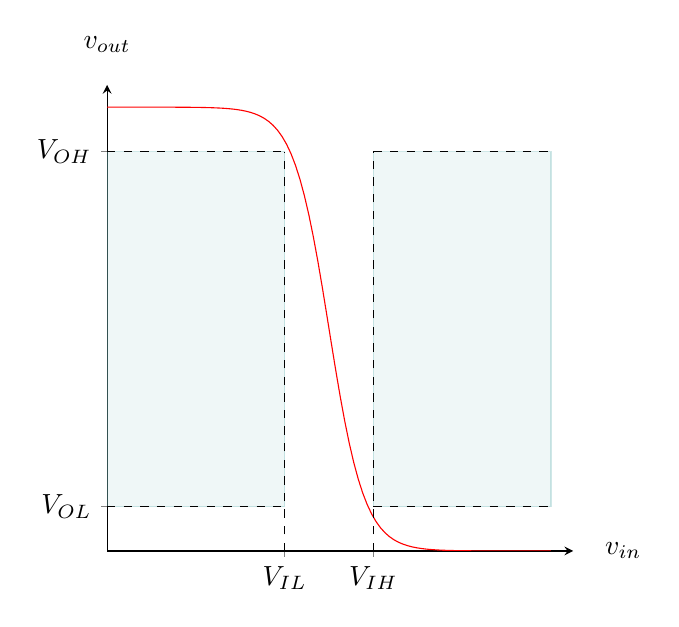
\begin{tikzpicture}
                        \begin{axis}[
                            xmin = 0, xmax = 5.25, % Axis Coordenates
                            ymin = 0, ymax = 5.25, % Axis Coordenates
                            xlabel = {$v_{\text{in}}$},  % Axis Labels
                            ylabel = {$v_{\text{out}}$}, % Axis Labels
                            xtick = {2,3},      % Axis Ticks Potions
                            ytick = {0.5,4.5},  % Axis Ticks Potions
                            xticklabels = {$V_{IL}$, $V_{IH}$}, % Axis Ticks Labels
                            yticklabels = {$V_{OL}$, $V_{OH}$}, % Axis Ticks Labels
                            x label style = {at={(axis cs:{5.5,0})}, anchor=west},
                            y label style = {at={(axis cs:{0,5.5})}, anchor=south, rotate=-90},
                            width  = 7.5cm,
                            height = 7.5cm,
                            % grid = both,
                            % grid style       = {line width=.1pt, draw=gray!10},
                            % major grid style = {line width=.2pt, draw=gray!50},
                            % minor tick num=1,
                            axis lines = left,
                        ]
                        \addplot [
                                domain=0:5, 
                                samples=100, 
                                color=red,
                        ] {5/(1+exp(+5*x-12.5))};
                        \draw[
                            color   =teal!75,
                            fill    =teal!25,
                            opacity =0.25
                        ] (3,0.5) rectangle (5, 4.5);
                        \draw[
                            color   =teal!75,
                            fill    =teal!25,
                            opacity =0.25
                        ] (0,0.5) rectangle (2, 4.5);
                        \draw[dashed] (axis cs:{2,0}) -- (axis cs:{2,4.5});
                        \draw[dashed] (axis cs:{3,0}) -- (axis cs:{3,4.5});
                        \draw[dashed] (axis cs:{0,0.5}) -- (axis cs:{2,0.5});
                        \draw[dashed] (axis cs:{3,0.5}) -- (axis cs:{5,0.5});
                        \draw[dashed] (axis cs:{0,4.5}) -- (axis cs:{2,4.5});
                        \draw[dashed] (axis cs:{3,4.5}) -- (axis cs:{5,4.5});
                        \end{axis}
                    \end{tikzpicture}
                \end{figure}\noindent
            Note que este gráfico não apresenta informações dinâmicas sobre o componente, isto é, não apresenta a velocidade para se atigir o regime. Além disso, as regiões coloridas representam as \textbf{Zonas Proíbidas}, não deverá haver sinal nestas regiões.

    \section{Sistemas Numéricos}
        \paragraph{Apresentação}Há diferentes formas para se representar números utilizadas em situações distintas de acordo com as necessidades da aplicação, sendo os principais sistemas serão apresentadas a seguir e comparados com o \textbf{Sistema Decimal}.

        \subsection{Binário}
            \paragraph{Definição}Sistema numérico que utiliza 2 dígitos: \{0,1\}, sendo que com $n$ bits o maior número possível representável será $2^{n}-1$ apresentando as seguintes posições especiais:
                \begin{enumerate}[noitemsep]
                    \item \textbf{LSB:} Least Significative Bit, bit mais à direita;
                    \item \textbf{MSB:} Most Significative Bit, bit mais à esquerda;
                \end{enumerate}
            Neste sistema será possível representar números fracionários através de potências negativas de 2 que apresenta manipulação similar as entradas inteiras.
                \begin{example}
                    Representação de Números Binários em Decimal:
                        \begin{table}[H]
                            \centering  
                            \begin{tabular}[]{r lll c rrr l}
                                $\dots$ & $2^3$ & $2^2$ & $2^1$ & $2^0$ & $2^{-1}$ & $2^{-2}$ & $2^{-3}$ & $\dots$\\\hline
                                        & 8     & 4     & 2     & 1     & 0.5      & 0.25     & 0.125    & \\
                            \end{tabular}
                            \caption{Representação de Números Binários}
                        \end{table}\noindent
                    Desta forma, sabe-se que:
                        \begin{equation*}
                            \boxed{
                                1011.010_{2} = 
                                1 \times 2^{ 3} + 
                                0 \times 2^{ 2} + 
                                1 \times 2^{ 1} + 
                                1 \times 2^{ 0} + 
                                0 \times 2^{-1} + 
                                1 \times 2^{-2}
                                 = 
                                 11.25_{10}
                            }
                        \end{equation*}
                \end{example}

            \paragraph{Soma Binária}Apresenta mesmo funcionamento para o sistema decimal como apresentado pelas seguintes tabelas:
                \begin{table}[H]
                    \centering  
                    \begin{tabular}[]{cc|cc}\hline
                        Soma & \texttt{Carry-In} & Resultado & \texttt{Carry-In}\\\hline
                        0 + 0 & 0 & 0 & 0\\
                        0 + 1 & 0 & 1 & 0\\
                        1 + 0 & 0 & 1 & 0\\
                        1 + 1 & 0 & 0 & 1\\
                        0 + 0 & 1 & 1 & 0\\
                        0 + 1 & 1 & 0 & 1\\
                        1 + 0 & 1 & 0 & 1\\
                        1 + 1 & 1 & 1 & 1\\\hline
                    \end{tabular}
                    \caption{Representação de Soma}
                \end{table}\noindent
            Onde:
                \begin{enumerate}[noitemsep]
                    \item \texttt{Carry-In:} Representa o acúmulo de entrada da operação anterior;
                    \item \texttt{Carry-Out:} Representa o acúmulo de saída da operação atual;
                \end{enumerate}

            \paragraph{Multiplicação Binária}Apresenta funcionamento próximo para o sistema decimal apresentando uma análise mais mecânica através da técnica de \texttt{shift-and-sum}, seguindo as seguintes regras:
                \begin{example}
                    Representação de $1101_{2} \times 1011_{2}$:
                    \begin{center}
                        \begin{arithmetic}
                                   1101 & \\
                            \times 1011 & \\
                                   1101 & 1, copia\\
                                  1101~ & 1, copia\\
                                 0000~~ & 0, anula\\
                            +   1101~~~ & 1, copia\\
                               10001111 & Resultado
                        \end{arithmetic}
                    \end{center}
                \end{example}

        \subsubsection{Conversão Decimal-Binário}
            \paragraph{Definição}Há dois principais métodos:
                \begin{enumerate}[noitemsep]
                    \item \textbf{Método de Inspeção:} Decompondo os números em soma de potências de 2;
                    \item \textbf{Método de Divisão Sucessiva:} Realizando divisões sucessivas de 2;
                \end{enumerate}
                \begin{example}
                    Método de Divisão Sucessiva:
                    \begin{figure}[H]
                        \centering
                        \basetenconversiontable{8}{2}
                        \caption{Conversão Decimal-Binário}
                    \end{figure}
                \end{example}

        \subsubsection{Complemento de 2}
            \paragraph{Definição}Representação de números negativos em binário a partir de sua representação positiva de tal forma que a soma seja sempre zero, obtido através de 2 métodos:
                \begin{enumerate}[rightmargin = \leftmargin]
                    \item \textbf{Método Básico:}
                        \begin{enumerate}[noitemsep]
                            \item Parte-se da representação positiva;
                            \item Inverte-se a representação;
                            \item Soma-se um a representação;
                        \end{enumerate}

                    \item \textbf{Método Rápido:}
                        \begin{enumerate}[noitemsep]
                            \item Parte-se da representação positiva;
                            \item Percorre o número da direita para esquerda até encontrar 1;
                            \item Invere-se os \texttt{bits} a esquerda do 1;
                        \end{enumerate}
                \end{enumerate}
                \begin{example}
                    Representação de Números Binários em Decimal:
                        \begin{table}[H]
                            \centering  
                            \begin{tabular}[]{cc cc cc cc}
                                $-2^7$ & $2^6$ & $2^5$ & $2^4$ & $2^3$ & $2^2$ & $2^1$ & $2^0$\\\hline
                                -128   & 64    & 32    & 16    & 8     & 4     & 2     & 1\\
                            \end{tabular}
                        \end{table}
                \end{example}
            Nota-se que nesta configuração será necessário ajustar as demais entradas em função da negativa para obter os números negativos desejados.

            \paragraph{Erros}Fisicamente o circuito utilizado para realizar a soma e a subtração será o mesmo e portanto haverá possibilidade de operações incosistentes pelas limitações da representação, apontadas pelos seguintes \texttt{Flags}:
                \begin{enumerate}
                    \item \textbf{Carry:} Erro na operação em números não sinalizados;
                        \begin{enumerate}
                            \item \texttt{Condição:}Acionada caso haja \texttt{mais um} na adição do \texttt{MSB};
                        \end{enumerate}

                    \item \textbf{Overflow:} Erro na operação em números em complemento de 2;
                        \begin{enumerate}
                            \item \texttt{Condição:}Resultado do \texttt{mais um} na adição do \texttt{MSB} diferentes das entradas;
                        \end{enumerate}
                \end{enumerate}

            \subsubsection{Representação Ponto Flutuante}
                \paragraph{Definição}Convenção numérica adequada proposta pelo IEEE para representação de números grandes ou pequenos representado na seguinte convenção:
                    \begin{figure}[H]
                        \centering
                        \begin{tikzpicture}
                            \draw[{Latex[round]}-{Latex[round]}] (0,1.5) -- (9,1.5) node[midway, yshift=0.25cm] {32 bits};
                    
                            \draw[color=black] 
                            (0,0) rectangle (1, 1) node[midway] {S};
                    
                            \draw[color=black] 
                            (1,0) rectangle (5, 1) node[midway] {E};
                    
                            \draw[color=black] 
                            (5,0) rectangle (9, 1) node[midway] {M};
                    
                            \node[black] at (0.5,-0.5) {1 bit};
                            \node[black] at (  3,-0.5) {8 bits};
                            \node[black] at (  7,-0.5) {23 bits};
                        \end{tikzpicture}
                    \end{figure}\noindent
                Obtido pela seguinte equação:
                    \begin{equation}
                        \boxed{
                            X_{10} = (-1)^{S}\times(1+M)\times 2^{E-127}
                        }
                    \end{equation}
                Onde:
                    \begin{enumerate}[noitemsep]
                        \item $S$, \texttt{bit de sinal};
                        \item $E$, \texttt{expoente polarizado};
                        \item $M$, \texttt{mantisa};
                    \end{enumerate}

    \section{Portas Lógicas}
        \begin{definition}
            Implementação de uma \textbf{Função Booleana} com pelo menos uma entrada e apenas uma saída.
        \end{definition}

        \subsection{Porta NOT}
            \begin{definition}
                Considera-se as seguintes características:
                \begin{multicols}{3}
                    \begin{table}[H]
                        \centering  
                        \begin{tabular}[]{c|c}\hline
                            in & out\\\hline
                            0  & 1\\
                            1  & 0\\\hline
                        \end{tabular}
                    \end{table}
                    \columnbreak\noindent
                        \begin{equation}
                            \boxed{
                                S = \overline{A}
                            }
                        \end{equation}
                    \columnbreak\noindent
                    \begin{figure}[H]
                        \centering
                        \begin{circuitikz}
                            \ctikzset{component text=left}
                            \draw
                            (0,0) node[not port] (myPort) {}
                            (myPort.in)  node [anchor = east] {in}
                            (myPort.out) node [anchor = west] {out};
                        \end{circuitikz} 
                    \end{figure}\noindent
                \end{multicols}\noindent
                Implementada a nível de software através da seguinte expressão:
                \begin{scriptsize}
                    \myStyleVHDL
                    \begin{lstlisting}
        S <= not A;
                    \end{lstlisting}
                \end{scriptsize}
            \end{definition}

        \subsection{Porta AND}
            \begin{definition}
                Considera-se as seguintes características:
                \begin{multicols}{3}
                    \begin{table}[H]
                        \centering  
                        \begin{tabular}[]{cc|c}\hline
                            A & B & out\\\hline
                            0 & 0 & 0\\
                            0 & 1 & 0\\
                            1 & 0 & 0\\
                            1 & 1 & 1\\\hline
                        \end{tabular}
                    \end{table}
                    \columnbreak\noindent
                        \begin{equation}
                            \boxed{
                                S = A \cdot B
                            }
                        \end{equation}
                    \columnbreak\noindent
                    \begin{figure}[H]
                        \centering
                        \begin{circuitikz}
                            \ctikzset{component text=left}
                            \draw
                            (0,0) node[and port] (myPort) {}
                            (myPort.in 1)  node [anchor = east] {A}
                            (myPort.in 2)  node [anchor = east] {B}
                            (myPort.out) node [anchor = west] {out};
                        \end{circuitikz} 
                    \end{figure} \noindent
                \end{multicols}\noindent
                Implementada a nível de software através da seguinte expressão:
                \begin{scriptsize}
                    \myStyleVHDL
                    \begin{lstlisting}
        S <= A and B;
                    \end{lstlisting}
                \end{scriptsize}
            \end{definition}

        \subsection{Porta NAND}
            \begin{definition}
                Considera-se as seguintes características:
                \begin{multicols}{3}
                    \begin{table}[H]
                        \centering  
                        \begin{tabular}[]{cc|c}\hline
                            A & B & out\\\hline
                            0 & 0 & 1\\
                            0 & 1 & 1\\
                            1 & 0 & 1\\
                            1 & 1 & 0\\\hline
                        \end{tabular}
                    \end{table}
                    \columnbreak\noindent
                        \begin{equation}
                            \boxed{
                                \overline{AB} = \overline{A} + \overline{B}
                            }
                        \end{equation}
                    \columnbreak\noindent
                    \begin{figure}[H]
                        \centering
                        \begin{circuitikz}
                            \ctikzset{component text=left}
                            \draw
                            (0,0) node[nand port] (myPort) {}
                            (myPort.in 1)  node [anchor = east] {A}
                            (myPort.in 2)  node [anchor = east] {B}
                            (myPort.out) node [anchor = west] {out};
                        \end{circuitikz} 
                    \end{figure} \noindent
                \end{multicols}\noindent
                Implementada a nível de software através da seguinte expressão:
                \begin{scriptsize}
                    \myStyleVHDL
                    \begin{lstlisting}
        S <= A nand B;
                    \end{lstlisting}
                \end{scriptsize}
            \end{definition}

        \subsection{Porta OR}
            \begin{definition}
                Considera-se as seguintes características:
                \begin{multicols}{3}
                    \begin{table}[H]
                        \centering  
                        \begin{tabular}[]{cc|c}\hline
                            A & B & out\\\hline
                            0 & 0 & 0\\
                            0 & 1 & 1\\
                            1 & 0 & 1\\
                            1 & 1 & 1\\\hline
                        \end{tabular}
                    \end{table}
                    \columnbreak\noindent
                        \begin{equation}
                            \boxed{
                                S = A + B
                            }
                        \end{equation}
                    \columnbreak\noindent
                    \begin{figure}[H]
                        \centering
                        \begin{circuitikz}
                            \ctikzset{component text=left}
                            \draw
                            (0,0) node[or port] (myPort) {}
                            (myPort.in 1)  node [anchor = east] {A}
                            (myPort.in 2)  node [anchor = east] {B}
                            (myPort.out) node [anchor = west] {out};
                        \end{circuitikz} 
                    \end{figure} \noindent
                \end{multicols}\noindent
                Implementada a nível de software através da seguinte expressão:
                \begin{scriptsize}
                    \myStyleVHDL
                    \begin{lstlisting}
        S <= A or B;
                    \end{lstlisting}
                \end{scriptsize}
            \end{definition}

        \subsection{Porta NOR}
           \begin{definition}
                Considera-se as seguintes características:
                \begin{multicols}{3}
                    \begin{table}[H]
                        \centering  
                        \begin{tabular}[]{cc|c}\hline
                            A & B & out\\\hline
                            0 & 0 & 1\\
                            0 & 1 & 0\\
                            1 & 0 & 0\\
                            1 & 1 & 0\\\hline
                        \end{tabular}
                    \end{table}
                    \columnbreak\noindent
                        \begin{equation}
                            \boxed{
                                \overline{A+B} = \overline{A} \cdot \overline{B}
                            }
                        \end{equation}
                    \columnbreak\noindent
                    \begin{figure}[H]
                        \centering
                        \begin{circuitikz}
                            \ctikzset{component text=left}
                            \draw
                            (0,0) node[nor port] (myPort) {}
                            (myPort.in 1)  node [anchor = east] {A}
                            (myPort.in 2)  node [anchor = east] {B}
                            (myPort.out) node [anchor = west] {out};
                        \end{circuitikz} 
                    \end{figure} \noindent
                \end{multicols}\noindent
                Implementada a nível de software através da seguinte expressão:
                \begin{scriptsize}
                    \myStyleVHDL
                    \begin{lstlisting}
        S <= A nor B;
                    \end{lstlisting}
                \end{scriptsize}
           \end{definition}

        \subsection{Porta XOR}
            \begin{definition}
                Considera-se as seguintes características:
                \begin{multicols}{3}
                    \begin{table}[H]
                        \centering  
                        \begin{tabular}[]{cc|c}\hline
                            A & B & out\\\hline
                            0 & 0 & 0\\
                            0 & 1 & 1\\
                            1 & 0 & 1\\
                            1 & 1 & 0\\\hline
                        \end{tabular}
                    \end{table}
                    \columnbreak\noindent
                        \begin{equation}
                            \boxed{
                                S = A \oplus B = A\overline{B} + \overline{A}B
                            }
                        \end{equation}
                    \columnbreak\noindent
                    \begin{figure}[H]
                        \centering
                        \begin{circuitikz}
                            \ctikzset{component text=left}
                            \draw
                            (0,0) node[xor port] (myPort) {}
                            (myPort.in 1)  node [anchor = east] {A}
                            (myPort.in 2)  node [anchor = east] {B}
                            (myPort.out) node [anchor = west] {out};
                        \end{circuitikz} 
                    \end{figure} \noindent
                \end{multicols}\noindent
                Implementada a nível de software através da seguinte expressão:
                \begin{scriptsize}
                    \myStyleVHDL
                    \begin{lstlisting}
        S <= A xor B;
                    \end{lstlisting}
                \end{scriptsize}
            \end{definition}

        \subsection{Porta XNOR}
            \begin{definition}
                Considera-se as seguintes características:
                \begin{multicols}{3}
                    \begin{table}[H]
                        \centering  
                        \begin{tabular}[]{cc|c}\hline
                            A & B & out\\\hline
                            0 & 0 & 1\\
                            0 & 1 & 0\\
                            1 & 0 & 0\\
                            1 & 1 & 1\\\hline
                        \end{tabular}
                    \end{table}
                    \columnbreak\noindent
                        \begin{equation}
                            \boxed{
                                S = \overline{A \oplus B}
                            }
                        \end{equation}
                    \columnbreak\noindent
                    \begin{figure}[H]
                        \centering
                        \begin{circuitikz}
                            \ctikzset{component text=left}
                            \draw
                            (0,0) node[xnor port] (myPort) {}
                            (myPort.in 1)  node [anchor = east] {A}
                            (myPort.in 2)  node [anchor = east] {B}
                            (myPort.out) node [anchor = west] {out};
                        \end{circuitikz} 
                    \end{figure} \noindent
                \end{multicols}\noindent
                Implementada a nível de software através da seguinte expressão:
                \begin{scriptsize}
                    \myStyleVHDL
                    \begin{lstlisting}
        S <= A xnor B;
                    \end{lstlisting}
                \end{scriptsize}
            \end{definition}

    \section{Álgebra Booleana}
        \begin{definition}
            Álgebra composta apenas por dois valores, geralmente são utilizados as seguinte notações:
                \begin{equation}
                    \boxed{\mathbb{B} = \{F, V\}}
                    \qquad
                    \boxed{\mathbb{B} = \{0, 1\}}
                \end{equation}
            Nota-se que os símbolos numéricos não possuem significado numérico nesta notação.
        \end{definition}

        \subsection{Opoerações Booleanas}
            \subsubsection{Axiomas}
            \begin{definition}
                Considera-se as seguintes operações como canônicas:
                    \begin{table}[H]
                        \centering  
                        \begin{tabular}[]{cc}\hline
                            $0\times0=0$ & $0+0=0$\\
                            $0\times1=0$ & $0+1=1$\\
                            $1\times0=0$ & $1+0=1$\\
                            $1\times1=1$ & $1+1=1$\\\hline
                            $\bar{0} =1$ & $\bar{1}=0$\\\hline
                        \end{tabular}
                        \caption{Axiomas Booleanos}
                    \end{table}
            \end{definition}
            \subsubsection{Teoremas}
            \begin{theorem}
                Considera-se que dada uma variável $x\in\mathbb{B}$ as seguintes operações serão válidas:
                    \begin{table}[H]
                        \centering  
                        \begin{tabular}[]{lcc}\hline
                            Aniquilação    & $x.0=0$ & $x+1=0$\\
                            Identidade     & $x.1=x$ & $x+0=x$\\
                            Idempotência   & $x.x=x$ & $x+x=x$\\
                            Complementação & $x.\bar{x}=0$ & $x+\bar{x}=1$\\\hline
                            Dupla Negação  & \multicolumn{2}{c}{$\bar{\bar{x}}=x$}\\\hline
                        \end{tabular}
                        \caption{Teoremas Booleanos de 1 Variável}
                    \end{table}
            \end{theorem}
            \begin{theorem}
                Considera-se que dadas três variáveis $x, y, z \in\mathbb{B}$ as seguintes operações serão válidas:
                    \begin{table}[H]
                        \centering  
                        \begin{tabular}[]{lcc}\hline
                            Comutatividade   & $x.y=y.x$          & $x+y=y+x$\\
                            Associatividade  & $x.(y.z)=(x.y).z$  & $x+(y+z)=(x+y)+z$\\
                            Distributividade & $x.(y+z)=x.y+x.z$  & $x+(y.z)=(x+y).(x+z)$\\
                            Absorção         & $x+xy=x$           & $x.(x+y)=x$\\
                            Combinação       & $xy+x\bar{y}=x$    & $(x+y).(x+\bar{y})=x$\\
                            Identidade Comum & $x.(\bar{x}+y)=xy$ & $x+(\bar{x}.y)=x+y$\\
                            DeMorgan         & $\overline{x.y}=\bar{x}+\bar{y}$ & $\overline{x+y}=\bar{x}.\bar{y}$\\\hline
                        \end{tabular}
                        \caption{Teoremas Booleanos de 2 Variáveis}
                    \end{table}
                Note que estes Teoremas de DeMorgan poderiam ser estendidos para qualquer conjunto finito de variáveis pertencentes ao conjunto $\mathbb{B}$ como enunciado a seguir:
                    \begin{enumerate}[noitemsep, rightmargin = \leftmargin]
                        \item \textbf{Complemento do Produto} de variáveis é igual à \textbf{Soma dos Complementos} das variáveis;
                        \item \textbf{Complemento da Soma} de variáveis é igual à \textbf{Produto dos Complementos} das variáveis;
                    \end{enumerate}
            \end{theorem}
        \subsubsection{Princípio da Dualidade}
            \begin{definition}
                Dual de uma expressão verdadeira é \textbf{sempre} verdadeira, sendo obtidas ao realizar as seguintes substituições:
                    \begin{equation}
                        \boxed{x \iff +}
                        \qquad
                        \boxed{0 \iff 1}
                    \end{equation}
            \end{definition}

    \section{Mapa de Karnaugh}
        \begin{definition}
            Organização geométrica das expressões obtidas pelas Tabelas Verdade de uma expressão booleana onde cada célula terá \textbf{Distância de Hamming} de 1 com relação as células vizinhas.
        \end{definition}
        \begin{theorem}
            Considera-se que para simplificar os sistemas as extremidades estarão conectadas. Desta forma, deve-se buscar a região que comporte o maior número de 1's agrupados em uma potência de 2.
        \end{theorem}
        \subsection{Mapa de Karnaugh, 2 Variáveis}
            \begin{definition}
                Considera-se a seguinte representado:
                    \begin{multicols}{2}
                        \begin{table}[H]
                            \centering
                            \begin{tabular}[]{cc|c}
                                $X_{1}$ & $X_{2}$ & \\\hline
                                0 & 0 & $m_{0}$\\
                                0 & 1 & $m_{1}$\\
                                1 & 0 & $m_{2}$\\
                                1 & 1 & $m_{3}$\\\hline
                            \end{tabular}
                            \caption{Tabela Verdade 2 Variáveis}
                        \end{table}
                        \columnbreak
                        \begin{figure}[H]
                            \centering
                            \begin{karnaugh-map}[2][2][1][$X_1$][$X_2$]
                                \terms{0}{$m_{0}$}
                                \terms{1}{$m_{2}$}
                                \terms{2}{$m_{1}$}
                                \terms{3}{$m_{3}$}
                            \end{karnaugh-map}
                            \caption{Mapa de Karnaugh 2 Variáveis}
                        \end{figure}
                    \end{multicols}
            \end{definition}
        \subsection{Mapa de Karnaugh, 3 Variáveis}
            \begin{definition}
                Considera-se a seguinte representado:
                    \begin{multicols}{2}
                        \begin{table}[H]
                            \centering
                            \begin{tabular}[]{ccc|c}
                                $X_1$ & $X_2$ & $X_3$& \\\hline
                                0     & 0     & 0    & $m_{0}$\\
                                0     & 0     & 1    & $m_{1}$\\
                                0     & 1     & 0    & $m_{2}$\\
                                0     & 1     & 1    & $m_{3}$\\
                                1     & 0     & 0    & $m_{4}$\\
                                1     & 0     & 1    & $m_{5}$\\
                                1     & 1     & 0    & $m_{6}$\\
                                1     & 1     & 1    & $m_{7}$\\\hline
                            \end{tabular}
                            \caption{Tabela Verdade 3 Variáveis}
                        \end{table}
                        \columnbreak
                        \begin{figure}[H]
                            \centering
                            \begin{karnaugh-map}[4][2][1][$X_1\;X_2$][$X_3$]
                                \terms{0}{$m_{0}$}
                                \terms{1}{$m_{2}$}
                                \terms{2}{$m_{4}$}
                                \terms{3}{$m_{6}$}
                                \terms{4}{$m_{1}$}
                                \terms{5}{$m_{3}$}
                                \terms{6}{$m_{5}$}
                                \terms{7}{$m_{7}$}
                            \end{karnaugh-map}
                            \caption{Mapa de Karnaugh 3 Variáveis}
                        \end{figure}
                    \end{multicols}
            \end{definition}
        \subsection{Mapa de Karnaugh, 4 Variáveis}
            \begin{definition}
                Considera-se a seguinte representado:
                    \begin{multicols}{2}
                        \begin{table}[H]
                            \centering
                            \begin{tabular}[]{cccc|c}
                                $X_1$ & $X_2$ & $X_3$ & $X_4$& \\\hline
                                0     & 0     & 0     & 0    & $m_{0}$\\
                                0     & 0     & 0     & 1    & $m_{1}$\\
                                0     & 0     & 1     & 0    & $m_{2}$\\
                                0     & 0     & 1     & 1    & $m_{3}$\\
                                0     & 1     & 0     & 0    & $m_{4}$\\
                                0     & 1     & 0     & 1    & $m_{5}$\\
                                0     & 1     & 1     & 0    & $m_{6}$\\
                                0     & 1     & 1     & 1    & $m_{7}$\\
                                1     & 0     & 0     & 0    & $m_{8}$\\
                                1     & 0     & 0     & 1    & $m_{9}$\\
                                1     & 0     & 1     & 0    & $m_{10}$\\
                                1     & 0     & 1     & 1    & $m_{11}$\\
                                1     & 1     & 0     & 0    & $m_{12}$\\
                                1     & 1     & 0     & 1    & $m_{13}$\\
                                1     & 1     & 1     & 0    & $m_{14}$\\
                                1     & 1     & 1     & 1    & $m_{15}$\\\hline
                            \end{tabular}
                            \caption{Tabela Verdade 4 Variáveis}
                        \end{table}
                        \columnbreak
                        \begin{figure}[H]
                            \centering
                            \begin{karnaugh-map}[4][4][1][$X_1\;X_2$][$X_3\;X_4$]
                                \terms{0}{$m_{0}$}
                                \terms{1}{$m_{4}$}
                                \terms{2}{$m_{8}$}
                                \terms{3}{$m_{12}$}
                                \terms{4}{$m_{1}$}
                                \terms{5}{$m_{5}$}
                                \terms{6}{$m_{9}$}
                                \terms{7}{$m_{13}$}
                                \terms{8}{$m_{2}$}
                                \terms{9}{$m_{6}$}
                                \terms{10}{$m_{10}$}
                                \terms{11}{$m_{14}$}
                                \terms{12}{$m_{3}$}
                                \terms{13}{$m_{7}$}
                                \terms{14}{$m_{11}$}
                                \terms{15}{$m_{15}$}
                            \end{karnaugh-map}
                            \caption{Mapa de Karnaugh 4 Variáveis}
                        \end{figure}
                    \end{multicols}
            \end{definition}
\end{document}